% Created 2024-02-05 Mon 22:21
% Intended LaTeX compiler: pdflatex
\documentclass[presentation]{beamer}
\usepackage[utf8]{inputenc}
\usepackage[T1]{fontenc}
\usepackage{graphicx}
\usepackage{longtable}
\usepackage{wrapfig}
\usepackage{rotating}
\usepackage[normalem]{ulem}
\usepackage{amsmath}
\usepackage{amssymb}
\usepackage{capt-of}
\usepackage{hyperref}
\mode<beamer>{\usetheme{Madrid}}
\definecolor{SUred}{rgb}{0.59375, 0, 0.17969} % SU red (primary)
\definecolor{SUblue}{rgb}{0, 0.17578, 0.38281} % SU blue (secondary)
\setbeamercolor{palette primary}{bg=SUred,fg=white}
\setbeamercolor{palette secondary}{bg=SUblue,fg=white}
\setbeamercolor{palette tertiary}{bg=SUblue,fg=white}
\setbeamercolor{palette quaternary}{bg=SUblue,fg=white}
\setbeamercolor{structure}{fg=SUblue} % itemize, enumerate, etc
\setbeamercolor{section in toc}{fg=SUblue} % TOC sections
% Override palette coloring with secondary
\setbeamercolor{subsection in head/foot}{bg=SUblue,fg=white}
\setbeamercolor{date in head/foot}{bg=SUblue,fg=white}
\institute[SU]{Shenandoah University}
\titlegraphic{
\includegraphics[width=0.5\textwidth]{\string~/Documents/suLogo/suLogo.pdf}}
\usetheme{default}
\author{Chase Mathison\thanks{cmathiso@su.edu}}
\date{6 February 2024}
\title{Volumes of Revolution: The Disk Method}
\hypersetup{
 pdfauthor={Chase Mathison},
 pdftitle={Volumes of Revolution: The Disk Method},
 pdfkeywords={},
 pdfsubject={},
 pdfcreator={Emacs 29.1 (Org mode 9.6.7)}, 
 pdflang={English}}
\begin{document}

\maketitle


\section{Announcements}
\label{sec:org0febb3d}
\begin{frame}[label={sec:org202add0}]{Announcements}
\begin{enumerate}
\item Homework!
\item Office hours!
\end{enumerate}
\end{frame}

\section{Volumes of revolution}
\label{sec:org7fef7db}
\begin{frame}[label={sec:org3cb44ca}]{Volumes of revolution}
One type of solid that comes up a lot in real life is a solid that is
generated by rotating a region about an axis.

One example of this is the unit sphere: it can be generate by rotating
a upper half circle of radius 1 and the area underneath it about the
\(x-\)axis. 

Really, any object that has circular cross sections can be generated
in this manner.  Because of this, what we learned last week will apply
to these \uline{\hspace*{1in}}. The volume of a solid of revolution
will be called a \uline{\hspace*{1in}}.

Let's look at a specific example before moving on to the general
method.
\end{frame}

\begin{frame}[label={sec:org19b16d9}]{Example}
Find the volume of the solid generated by rotating the region bounded
by the curves
\[
y = \frac{1}{x},\, x = 1,\, x = 2,\, y = 0 \]
about the \(x-\)axis by using the method of slicing.
\vspace{10in}
\end{frame}

\begin{frame}[label={sec:org00e9dd0}]{Example}
\end{frame}

\begin{frame}[label={sec:org36a554d}]{The disk method}
The main difference between what we're talking about today, and what
we talked about last time, is that we know beforehand with a solid of
revolution that the cross-sectional areas are going to be circles.

Let's look at a general curve, and the volume that results from it
when we rotate the region of interest about the \(x-\)axis:
\vspace{10in}
\end{frame}

\begin{frame}[label={sec:orgeb53302}]{The disk method}
\end{frame}

\begin{frame}[label={sec:orgdf17af4}]{The disk method}
We have shown the following
\begin{theorem}[The disk method]
Let \(f \left( x \right)\) be continuous and non-negative.  Let \(R\) be the region bounded above by the graph of \(f \left( x \right)\), below by the \(x-\)axis and by the curves \(x = a\) and \(x=b\).  Then, the volume of the solid that is generated by rotating \(R\) about the \(x-\)axis is given by
\[
\, \]
\phantom{butts}

\phantom{butts}
\end{theorem}
\end{frame}


\begin{frame}[label={sec:org46f8fa8}]{Example (Volume of a circular cone)}
Find the volume of the solid that is generated by rotating the region
in the first quadrant that is bounded above by \(y = -\frac{r}{h}x + r\)
about the \(x-\)axis, where \(r\) and \(h\) are constants.
\vspace{10in}
\end{frame}

\begin{frame}[label={sec:org418afcd}]{Example}
\end{frame}

\begin{frame}[label={sec:orga1943e0}]{Example}
Find the volume of the solid that is generated by rotating the region
bounded by the curves \(y = \sin \left( x \right)\), \(y = 0\), \(x
= 0\) and \(x = \pi\) about the \(x-\)axis.

\begin{center}
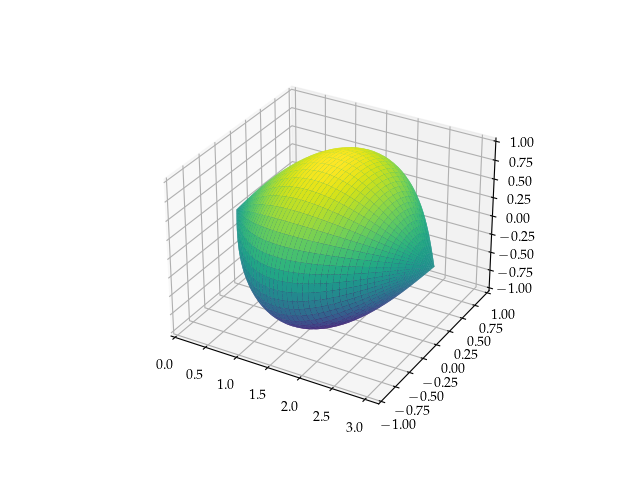
\includegraphics[width=0.5\textwidth]{../img/day006-ex01.png}
\end{center}
\vspace{10in}
\end{frame}

\begin{frame}[label={sec:org2c0d402}]{Example}
\end{frame}

\begin{frame}[label={sec:org773fb7f}]{Example}
Find the volume of the solid generated by rotating the region bounded
by the curves \(y = \sqrt{x}\), \(y = 0\), \(x = 0\) and \(x = 3\)
about the \(x-\)axis.

\begin{center}
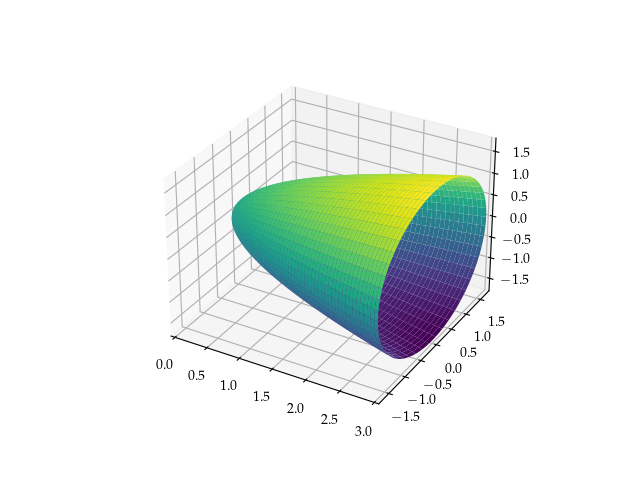
\includegraphics[width=0.5\textwidth]{../img/day006-ex02.png}
\end{center}
\vspace{10in}
\end{frame}

\begin{frame}[label={sec:org9777828}]{Example}
\end{frame}

\begin{frame}[label={sec:orge838e0f}]{The disk method for functions of \(y\)}
We can use this exact same method to find the volume of solids of
revolution generated by rotating regions about the \(y-\)axis.  
When we do this, we need to make sure to write our functions in terms
of \uline{\hspace*{1in}}.  This will give us the following rule: 

\begin{theorem}[Disk method (in terms of \(y\))]
Let \(g \left( y \right)\) be continuous and nonnegative. Defined \(Q\) to be the region bounded on the right by the graph of \(g \left( y
\right)\), on the left by \(x = 0\), and between \(y = c\) and \(y
= d\).  Then the volume of the solid generated by rotating \(Q\)
around the \(y-\)axis is given by
\[
\, \]
\phantom{butts}
\end{theorem}
\end{frame}

\begin{frame}[label={sec:orgaa01b44}]{Example}
Find the volume of the solid generated by rotating the region bounded
by the curves \(y = \sqrt{1 + x}\), \(x = 0\), and \(y = 2\) about
the \(y-\)axis.

\begin{center}
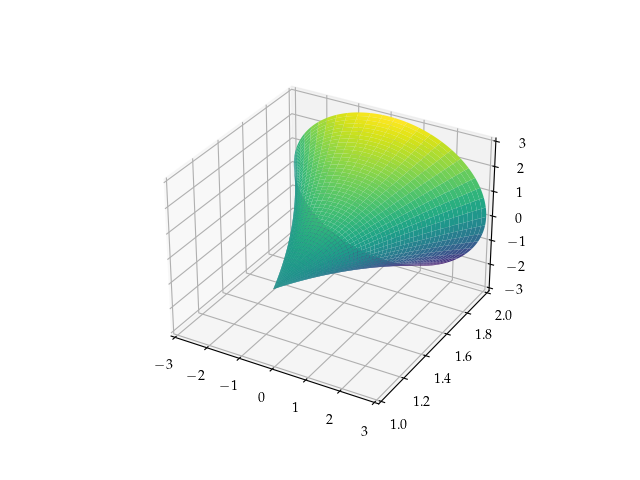
\includegraphics[width=0.5\textwidth]{../img/day006-ex03.png}
\end{center}
\vspace{10in}
\end{frame}

\begin{frame}[label={sec:org0e90eac}]{Example}
\end{frame}

\begin{frame}[label={sec:org5c019f9}]{Next time}
Next time we'll talk about how to find the volume of even more
complicated volumes of revolution using the \emph{washer method} (of which
the disk method is just a special case).

Make sure to get started on the homework!
\end{frame}
\end{document}